\documentclass[11pt]{article}

\usepackage{amsmath,amssymb,amsthm}
\usepackage{booktabs}
\usepackage{graphicx}
\usepackage[hyphens]{url}
\usepackage{hyperref}
\usepackage[margin=1in]{geometry}
\usepackage{enumitem}
\usepackage{microtype}

\urlstyle{tt}

\newtheorem{theorem}{Theorem}
\newtheorem{lemma}{Lemma}
\newtheorem{definition}{Definition}
\newtheorem{corollary}{Corollary}

\title{Exact Local Output Perturbation in KV-Cache Eviction:\\
Ranking Inversions and Their Downstream Consequences}
\author{Elias De Jesús\\
\small Independent Researcher\\
\small ORCID: 0009-0007-0190-9143}
\date{September 2026}

\begin{document}
\maketitle

\begin{abstract}
Deleting a token from a transformer's KV cache and renormalizing the surviving
attention weights changes a single attention head's output by an amount that
can be computed exactly, in closed form, before any downstream computation
occurs. This raises a natural question: if the immediate local effect of an
eviction decision is known exactly, how much does that exact local
information tell us about the model's eventual downstream behavior? We
derive a closed-form, necessary-and-sufficient boundary condition ($\Gamma$)
for when this exact local-perturbation ranking of eviction candidates
disagrees with the simpler attention-mass ranking, and show that such
disagreements are neither rare nor dominant, and that when they occur they
almost always change the eviction decision and produce a measurable
downstream effect, replicated across a GPT-NeoX/Pythia-160M and a GPT-2
(124M) grid. However, in a stratified, cluster-aware causal-tracing audit of
$250$ such cases, the token favored by the exact local metric at the moment
of eviction is overturned by later transformer blocks in roughly a third of
cases ($32.4\%$, 95\% CI $[26.1\%,39.2\%]$, cluster bootstrap), a rate not
reliably distinguishable between the two architectures we tested. A sequence
of falsification experiments --- static directional value-vector geometry,
propagation depth, logit-space representation, and state-dependent block
sensitivity --- fails to reduce this downstream behavior to a simple
predictor. We conclude that an exact, provably correct local measure of
eviction perturbation is not, by itself, a reliable guide to downstream
model behavior, and we characterize precisely where and how that gap arises.
The central identity underlying our local score is algebraically identical,
in its single-token case, to an equation independently derived by prior
KV-cache work \cite{keepkv2025}; our contribution is the pairwise
ranking-inversion boundary built on top of it and the empirical/causal study
of its downstream consequences, not the identity itself. All results are
established on two small-to-moderate autoregressive language models and a
deliberately stratified (not uniformly random) case sample; we make no claim
about larger or instruction-tuned models, and no claim about which eviction
policy one should deploy.
\end{abstract}

\section{Introduction}
\label{sec:intro}

Autoregressive transformer inference keeps a key-value (KV) cache of every
previously seen token so that later positions can attend to earlier ones
without recomputation. For long contexts this cache dominates memory use,
and a large body of work proposes \emph{eviction policies} that discard some
cached tokens to bound memory --- most commonly by ranking tokens according
to a cheap proxy of importance, such as accumulated attention mass
\cite{h2o2023,scissorhands2023,streamingllm2024}.

Attention mass alone does not fully specify what deleting a token actually
does to the head's output: a token can carry substantial mass yet sit close
to the aggregated output (so removing it barely moves anything), or carry
little mass yet sit far from it (so removing it, after renormalization,
moves the output by more than its mass alone would suggest). A different,
more exact question is available but has received comparatively little
attention: for a single attention head, deleting a token from the softmax
and renormalizing the remaining weights changes that head's output by an
amount that can be written down \emph{exactly}, in closed form, as a
function of the deleted token's attention weight \emph{and} its value
vector's displacement from the head's current output. This exact local
quantity is not a heuristic and not an approximation; it is an algebraic
identity. Because it depends on both quantities and attention-mass ranking
depends on only one, the two rankings need not agree; the boundary condition
$\Gamma$ we derive (Section~\ref{sec:gamma}) makes precise exactly when they
disagree, rather than leaving it as an empirical observation.

This paper asks a single, narrow question:

\begin{quote}
\emph{If the immediate effect of deleting a KV token can be computed
exactly, how much does that exact local information tell us about
downstream model behavior?}
\end{quote}

The answer we find, and defend with pre-registered, cluster-aware,
cross-architecture evidence, is:

\begin{quote}
It determines the local ranking exactly and yields an exact boundary for
disagreement with attention-mass ranking, but it does not reliably determine
the downstream winner after subsequent transformer blocks.
\end{quote}

\paragraph{What this paper is not.} This is not a new KV-cache eviction
algorithm, not a claim that any policy studied here is optimal, not a
benchmark comparison against deployed systems such as H$_2$O or SnapKV, not
a universal theorem about transformers in general, not an AI-safety
contribution, and not a claim that downstream transformer behavior is
chaotic or unpredictable. It is a precise, falsification-oriented
mechanistic study of the gap between an exact local perturbation measure and
downstream outcome.

\paragraph{Prior-art correction stated up front.} The single-token special
case of the exact identity we build on is algebraically identical to an
equation independently derived in concurrent KV-cache work, KeepKV
\cite{keepkv2025} (Section~\ref{sec:relatedwork},
Section~\ref{sec:localgeometry}). We state this explicitly here, rather than
leaving it for related work, because it determines what in this paper can be
claimed as new: not the identity, but the pairwise ranking-inversion
boundary derived from it (Section~\ref{sec:gamma}) and the empirical/causal
study of its downstream consequences (Sections~\ref{sec:consequences}
through \ref{sec:falsification}).

\paragraph{Contributions.}
\begin{enumerate}[nosep]
\item A closed-form, necessary-and-sufficient pairwise boundary condition
($\Gamma$) determining when an attention-mass ranking and an exact
local-output-perturbation ranking of two eviction candidates disagree
(Theorem~\ref{thm:gamma}). To our knowledge, no prior work derives this
condition.
\item A four-step, numerically verified empirical chain relating ranking
inversions to measurable downstream consequences, replicated across two
architectures (Section~\ref{sec:consequences}).
\item A cluster-aware causal-tracing audit ($n=250$ stratified cases)
showing that the immediate local-damage winner is overturned by downstream
computation in roughly one third of cases, with uncertainty estimated by a
cell-level cluster bootstrap rather than treating candidate pairs as
independent (Section~\ref{sec:downstream}).
\item A four-stage falsification sequence (static geometry, propagation
depth, functional/logit-space representation, state-dependent block
sensitivity) that fails to reduce this downstream behavior to a simple
predictor, including a positive causal finding (state-dependence exists) that
is nonetheless \emph{not} an explanation for the reversals
(Section~\ref{sec:falsification}).
\end{enumerate}

\section{Related Work}
\label{sec:relatedwork}

\paragraph{Exact eviction perturbation.} KeepKV \cite{keepkv2025} derives,
as an intermediate step toward a bound on merging-based KV compression, the
identity $o' = (o - \alpha_e v_e)/(1-\alpha_e)$ for the head output after a
single token $e$ is deleted and the remaining weights renormalized. As we
show in Section~\ref{sec:localgeometry}, this is algebraically identical to
the singleton case of the identity we use, $\Delta_i = \alpha_i(o-v_i)/(1-\alpha_i)$.
We do not claim this identity as new. KeepKV uses it operationally, inside
an EMA-based error bound for its merging procedure; it does not use it to
define a per-token ranking score, and it does not derive a ranking-inversion
condition against attention-mass ranking. Our block-$B$ generalization
(simultaneous multi-token eviction) is a direct linear extension of this
same substitution and is not presented as a separate contribution.

\paragraph{Attention-mass and heuristic eviction scoring.} H$_2$O
\cite{h2o2023} retains tokens by accumulated attention-mass ``heavy
hitters''; Scissorhands \cite{scissorhands2023} exploits persistence of
token importance across steps; StreamingLLM \cite{streamingllm2024}
identifies an attention-sink phenomenon at initial positions. We use
attention-mass ranking, in the spirit of this line of work, as one of the
two policies compared throughout this paper. We do not compare against
these systems empirically on downstream task quality; our comparison is
restricted to the two rankings themselves and their measured effect on
next-token KL divergence.

\paragraph{Value-aware and bound-based scoring.} CriticalKV \cite{criticalkv2025}
derives an upper \emph{bound} on output perturbation using an L1 value-state
norm, not an exact identity. A concurrent diagnostic framework
\cite{fixedcontract2026} scores candidates by squared distance to a
weighted-centroid approximation of the retained set's output, not the true
renormalized output. Neither derives an explicit ranking-inversion condition
between two named scoring rules; both are structurally related to, but not
equivalent to, the score we use (to our knowledge; see
Section~\ref{sec:localgeometry}).

\paragraph{Causal tracing and logit-space projection.} Our downstream
audits (Sections~\ref{sec:downstream}--\ref{sec:falsification}) apply
activation patching / causal-mediation analysis, in the sense established by
causal tracing of factual associations in GPT-style models
\cite{rome2022}, and logit-lens-style projection of intermediate hidden
states to vocabulary space, in the sense formalized by the Tuned Lens
\cite{tunedlens2023}. Both are established general techniques that we apply
to a specific, narrow question (does an eviction policy's local ranking
survive propagation); we do not claim either technique itself as a
contribution of this paper.

\section{Exact Local Eviction Geometry}
\label{sec:localgeometry}

\subsection{Setup}

For a single attention head, let $\alpha \in \mathbb{R}^n_{>0}$ be the
softmax attention-weight vector over $n$ keys, $\sum_k \alpha_k = 1$, and let
$v_k$ denote the value vector already mapped into the quantity that is
linearly combined to form the head's output (i.e.\ $v_k = W_O^h v_k^{\text{raw}}$
in the usual notation, so that the output is a plain weighted sum). The head
output is
\[
o = \sum_k \alpha_k v_k .
\]
For a block $B$ of tokens to be evicted, define the block mass, block
contribution, and residual
\[
m_B = \sum_{i \in B} \alpha_i, \qquad
o_B = \sum_{i \in B} \alpha_i v_i, \qquad
r_B = o_B - m_B \, o .
\]

\begin{theorem}[Exact delete-and-renormalize identity]
\label{thm:delta}
Deleting block $B$ from the softmax and renormalizing the surviving weights
to sum to $1$ changes the head output by exactly
\[
\Delta_B = \frac{m_B \, o - o_B}{1 - m_B} = -\frac{r_B}{1-m_B}, \qquad m_B < 1 .
\]
\end{theorem}

\begin{proof}
The renormalized output after deleting $B$ is
$o' = \sum_{k \notin B} \frac{\alpha_k}{1-m_B} v_k
= \frac{1}{1-m_B}\Big( \sum_k \alpha_k v_k - \sum_{i\in B} \alpha_i v_i \Big)
= \frac{o - o_B}{1-m_B}$.
Then $\Delta_B = o' - o = \frac{o - o_B}{1-m_B} - o = \frac{o - o_B - o(1-m_B)}{1-m_B}
= \frac{m_B o - o_B}{1-m_B}$, which equals $-r_B/(1-m_B)$ by definition of
$r_B$. \emph{This is direct algebraic substitution, not an approximation.}
\end{proof}

This identity, its proof, and the exclusion of the degenerate case
$m_B \to 1$ (where the renormalized output is undefined, not merely
ill-conditioned) are implemented and unit-tested in this project's code
(\url{src/kv_efficiency/local_algebra.py}), independent of model
architecture.

\subsection{Prior-art correction: the singleton case is not new}
\label{sec:priorart}

For a single evicted token $i$ ($B=\{i\}$), $m_B = \alpha_i$ and
$o_B = \alpha_i v_i$, so Theorem~\ref{thm:delta} specializes to
\[
\Delta_i = \frac{\alpha_i(o - v_i)}{1-\alpha_i}. \tag{$\ast$}
\]
KeepKV \cite{keepkv2025} derives, for the output after deleting a single
token $e$ and renormalizing, $o' = (o - \alpha_e v_e)/(1-\alpha_e)$. Taking
$o' - o$:
\[
o'-o = \frac{o-\alpha_e v_e}{1-\alpha_e} - o
= \frac{\alpha_e o - \alpha_e v_e}{1-\alpha_e}
= \frac{\alpha_e(o-v_e)}{1-\alpha_e},
\]
which is line-for-line identical to $(\ast)$, including sign. \textbf{We
state plainly that the singleton exact-perturbation identity is not a novel
contribution of this paper.} It is cited here, and used, but not claimed as
new. Our block-$B$ form (Theorem~\ref{thm:delta}) is a direct linear
generalization to simultaneous multi-token eviction; we present it as an
extension, not a separate result.

\subsection{Exact local output perturbation}

\begin{definition}[Exact local output perturbation]
For a single candidate token $i$, define
\[
d_i = \frac{\alpha_i}{1-\alpha_i}\,\|o - v_i\| = \|\Delta_i\| .
\]
\end{definition}

$d_i$ is the exact Euclidean norm of the change in \emph{one attention
head's output}, computed before any downstream transformation, caused by
deleting token $i$ from the softmax and renormalizing the surviving weights.
We use \textbf{exact local output perturbation} as the primary term for
$d_i$ throughout this paper. It is not global damage, not downstream
importance, not causal importance in the sense of Section~\ref{sec:relatedwork}'s
causal-tracing literature, and not an optimality claim of any kind; each of
those would require evidence this paper explicitly does not claim to
provide, and indeed the results of Sections~\ref{sec:downstream}--\ref{sec:falsification}
show that $d_i$ does not reliably predict several of them.

\section{Pairwise Ranking-Inversion Boundary}
\label{sec:gamma}

Attention-mass ranking orders candidates by $\alpha_i$ alone. Exact local
output perturbation orders them by $d_i = [\alpha_i/(1-\alpha_i)] \, g_i$,
$g_i := \|o - v_i\|$. These two rankings need not agree, because $d_i$ also
depends on $g_i$, which attention-mass ranking ignores entirely. We derive
the exact condition under which they disagree.

\begin{theorem}[Pairwise ranking-inversion boundary]
\label{thm:gamma}
Let $i,j$ be candidates with $0 < \alpha_i < \alpha_j < 1$ and $g_i, g_j > 0$.
Define
\[
G_{ij} = \frac{g_i}{g_j}, \qquad
M_{ij} = \frac{\alpha_j(1-\alpha_i)}{\alpha_i(1-\alpha_j)}, \qquad
\Gamma_{ij} = \log G_{ij} - \log M_{ij} .
\]
Then
\[
d_i > d_j \iff G_{ij} > M_{ij} \iff \Gamma_{ij} > 0,
\]
and symmetrically with $=$ and $<$.
\end{theorem}

\begin{proof}
$d_i > d_j \iff \frac{\alpha_i}{1-\alpha_i} g_i > \frac{\alpha_j}{1-\alpha_j} g_j$.
All four quantities $\alpha_i, \alpha_j, 1-\alpha_i, 1-\alpha_j$ are strictly
positive by hypothesis ($0<\alpha_i<\alpha_j<1$), as are $g_i,g_j$, so the
inequality is preserved on dividing both sides by $\frac{\alpha_j}{1-\alpha_j}g_j > 0$:
\[
d_i > d_j \iff \frac{g_i}{g_j}\cdot\frac{\alpha_i(1-\alpha_j)}{\alpha_j(1-\alpha_i)} > 1
\iff G_{ij} > M_{ij}.
\]
Since both $G_{ij}$ and $M_{ij}$ are strictly positive, $\log$ is a strictly
increasing bijection on $(0,\infty)$, so $G_{ij} > M_{ij} \iff \log G_{ij} >
\log M_{ij} \iff \Gamma_{ij} > 0$. The equality and reverse cases follow
identically with $=$ and $<$.
\end{proof}

\begin{figure}[t]
\centering
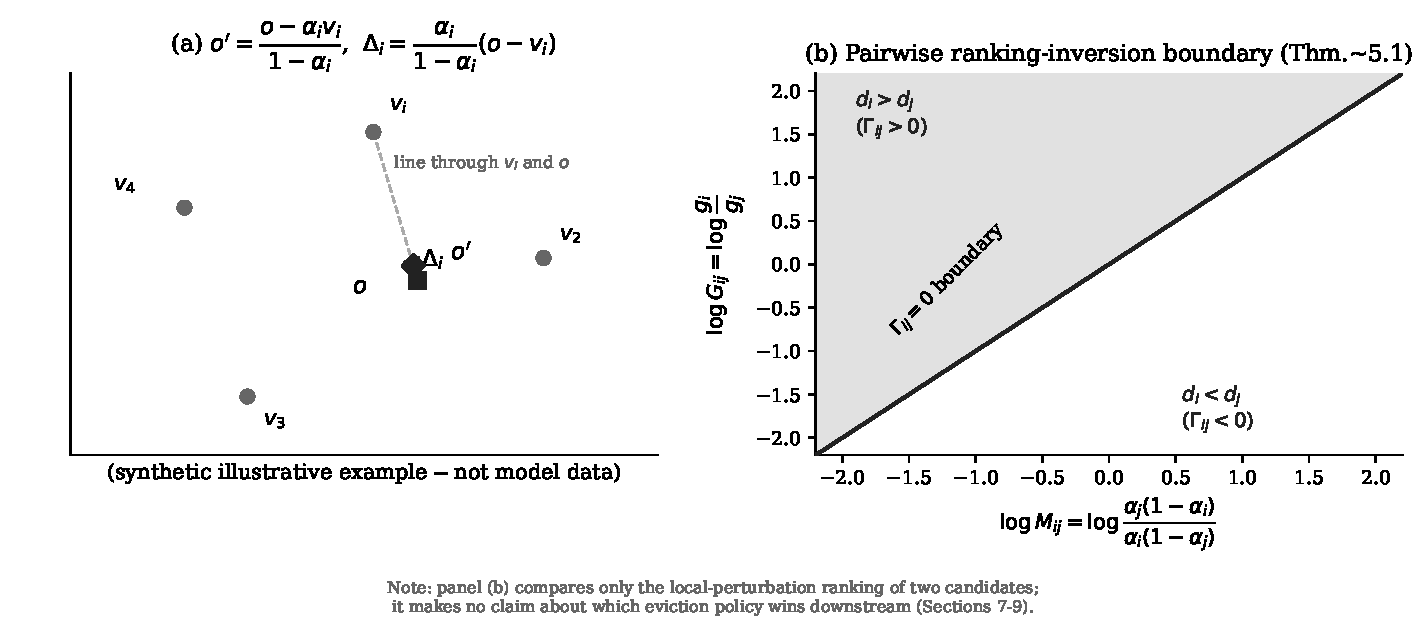
\includegraphics[width=\textwidth]{figures/fig1_local_perturbation_gamma.pdf}
\caption{(a) A schematic, synthetic example (not model data) of the exact
delete-and-renormalize geometry of Theorem~\ref{thm:delta}: deleting token
$i$ moves the head output from $o$ to $o'$ along the line through $v_i$ and
$o$, by exactly $\Delta_i = [\alpha_i/(1-\alpha_i)](o-v_i)$. (b) The
$\Gamma_{ij}=0$ boundary of Theorem~\ref{thm:gamma} in the
$(\log M_{ij}, \log G_{ij})$ plane. Panel (b) compares only which of two
candidates has the larger exact local perturbation; it makes no claim about
which eviction policy produces the smaller downstream KL divergence, a
separate, empirically measured question addressed in
Sections~\ref{sec:consequences}--\ref{sec:falsification}.}
\label{fig:local-gamma}
\end{figure}

Figure~\ref{fig:local-gamma} illustrates both the geometry of
Theorem~\ref{thm:delta} and the boundary condition of
Theorem~\ref{thm:gamma}.

\paragraph{Equality case.} $\Gamma_{ij}=0$ is the exact boundary at which the
distance ratio $G_{ij}$ exactly compensates the mass-ratio term $M_{ij}$;
on this boundary the two rankings agree in outcome even though they measure
different quantities.

\paragraph{Edge cases.} As $\alpha_i \to 0$, $d_i \to 0$ regardless of
$g_i$: a vanishing-mass token does vanishing damage on removal, consistent
with the identity, not an exception to it. The case $\alpha_i \to 1$ is
excluded by hypothesis and by Theorem~\ref{thm:delta} (the renormalized
output is undefined when a block carries essentially all the mass). When
$\alpha_i = \alpha_j$, $M_{ij}=1$ and $\Gamma_{ij} = \log(g_i/g_j)$: the
mass term drops out and the comparison reduces to comparing $g_i,g_j$
directly, as expected. When $g_i=0$ or $g_j=0$ (a candidate whose value
vector coincides exactly with the head output), $d_i=0$ or $d_j=0$
trivially and $\log G_{ij}$ is undefined; the underlying (non-log)
comparison $G_{ij}>M_{ij}$ remains well defined and should be used directly
in this degenerate case.

\paragraph{Are logarithms necessary?} No. The decisive statement is the
ratio comparison $G_{ij}>M_{ij}$; $\Gamma_{ij}$ is a monotone
reparametrization chosen for numerical convenience (differences of logs
avoid over/underflow when masses or distances are extreme, and give the
boundary the natural form $\Gamma_{ij}=0$). $\Gamma_{ij}$ carries no
mathematical content beyond $G_{ij}$ and $M_{ij}$ themselves.

\emph{No claim of novelty is made within this theorem statement or proof;
the novelty assessment for this result is given in Section~\ref{sec:relatedwork}
and stated cautiously there (``to our knowledge'').}

\section{Experimental Design and Validated Architecture Adapters}
\label{sec:design}

We evaluate all claims on two architectures: GPT-NeoX/Pythia-160M (parallel
attention/MLP residual structure) and GPT-2 (124M) (sequential residual
structure, Conv1D-based attention). To recompute exact per-head attention
weights, value vectors, and outputs identically across both, we built two
validated adapters exposing a shared contract
(\url{src/kv_efficiency/attention_reconstruction*.py}). The GPT-2
adapter (new to this project) is validated by 8 dedicated unit tests plus
inline numerical checks against a pilot grid (36 prompt$\times$layer$\times$head
cells): row-sum deviation from 1 up to $3.28\times10^{-7}$, zero causal
leakage, query/key recomputation error up to $3.27\times10^{-7}$, $c\_proj$
reconstruction relative error up to $1.97\times10^{-7}$, and
delete-and-renormalize identity error up to $2.84\times10^{-14}$ across 180
checks, all attributable to ordinary float32 accumulation, not an
implementation defect. The full project test suite (74 tests, all passing
at time of writing) includes these 8 GPT-2-adapter tests alongside the
pre-existing architecture-independent local-algebra tests. This pilot grid
is used exclusively for adapter validation in this paper; its own
inversion-prevalence figures are not used as a headline empirical result
anywhere in this manuscript (see Section~\ref{sec:consequences} and
Appendix~\ref{app:supplement} for the two grids that are).

Two grids were computed: a Pythia-160M grid (5 layers $\times$ 4 heads
$\times$ 3 prompts, 55{,}971 total candidate pairs) and a GPT-2 full grid
(12 layers $\times$ 12 heads $\times$ 3 prompts, 426{,}816 total candidate
pairs). In both, every computed $\Gamma_{ij}$ value was independently
cross-checked against direct recomputation of $d_i,d_j$ from the underlying
$\alpha,v$ data: $0$ mismatches in $55{,}971$ checks (Pythia) and $0$
mismatches in $426{,}816$ checks (GPT-2). This is a sanity check on the
implementation of Theorem~\ref{thm:gamma}, not evidence for any empirical
claim.

\begin{small}
\paragraph{Reproducibility.} Pythia was loaded as
\url{EleutherAI/pythia-160m} pinned to git revision
\texttt{50f5173d932e} (12-character prefix of the full 40-character SHA
recorded in the stored run provenance); GPT-2 was loaded as the unpinned
Hugging Face \texttt{gpt2} checkpoint (no revision was pinned for GPT-2 in the
underlying experiment code, unlike Pythia -- noted here rather than
obscured). Every stratified draw and bootstrap resample in this paper (the
250-case sample of Section~\ref{sec:downstream}, its cluster bootstrap, and
the SDPH case selection of Section~\ref{sec:falsification}) uses the fixed
seed $20{,}260{,}910$. Every \texttt{results} directory cited in this paper has a corresponding,
identically named script under \texttt{experiments/} in the project
repository that produced it (for example,
\url{results/downstream_propagation_sample/} is produced by
\url{experiments/downstream_propagation_sample.py}). Exact prompt texts and
grid configuration are recorded in \texttt{configs/milestone2\_grid.yaml}.
\end{small}

\section{Ranking Inversions and Their Immediate Consequences}
\label{sec:consequences}

We report four logically separate empirical statements, verified against
the stored grid outputs and kept deliberately un-merged, since each has a
different (and generally weaker, moving down the list) evidential strength.

\begin{enumerate}[label=(\arabic*),nosep]
\item \textbf{Attention-mass and exact-local-perturbation rankings sometimes
invert.} Meaningful inversions ($\Gamma_{ij}\neq 0$ under the pre-declared
floors) occur in $1{,}987/55{,}971 = 3.55\%$ of Pythia candidate pairs and
$22{,}983/426{,}816 = 5.38\%$ of GPT-2 candidate pairs. The two grids are
not equally dense or directly comparable (different layer/head coverage,
different candidate-pool sizes per cell), so this prevalence difference
should not be over-interpreted as an architecture effect; both figures show
the same qualitative fact, that inversions are neither vanishingly rare nor
dominant.
\item \textbf{Inversions almost always change the eviction selection.} Among
these inversions, the evicted token set actually changes within the
candidate range in $99.60\%$ of Pythia cases and $99.57\%$ of GPT-2 cases.
\item \textbf{Changed selections almost always produce a measurable
downstream KL difference.} Among set-changing inversions, the resulting
final-layer KL divergence exceeds the pre-declared, diagnostically justified
noise floor in $99.14\%$ of Pythia cases and $98.22\%$ of GPT-2 cases.
\emph{Measurable} here means only ``above the configured numerical
threshold,'' not necessarily practically large; advantage magnitudes span
several orders of magnitude (Pythia interquartile range of $|\text{advantage}|$
spans from $\sim 10^{-6}$ to $\sim 10^{-2}$; see stored percentile data).
\item \textbf{The locally preferred choice does not reliably remain the
final downstream winner.} This is the subject of Section~\ref{sec:downstream}
and is \emph{not} implied by (1)--(3).
\end{enumerate}

\begin{figure}[t]
\centering
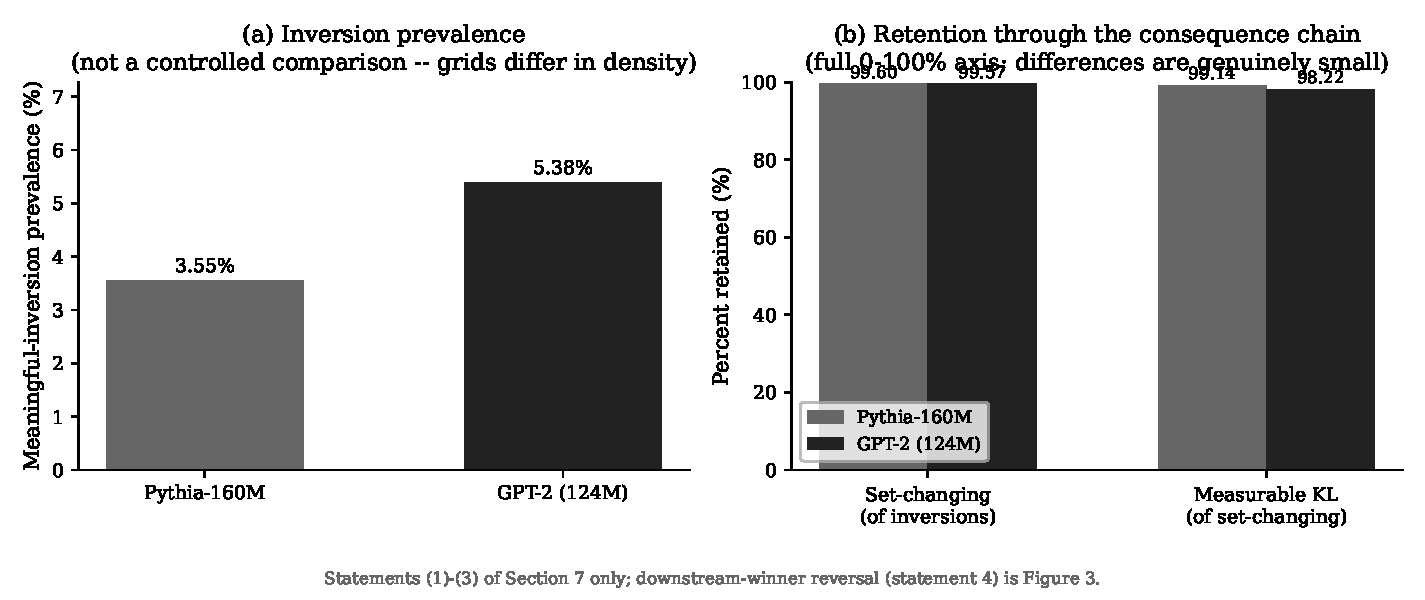
\includegraphics[width=\textwidth]{figures/fig2_inversion_chain.pdf}
\caption{Statements (1)--(3) above, computed directly from the stored grid
outputs (\url{results/full_grid_mechanistic_analysis/} for Pythia,
\url{results/cross_architecture_full_grid/} for GPT-2; see
\url{manuscript/figures/FIGURE_PROVENANCE.md} for the exact keys and
filters). (a) Meaningful-inversion prevalence on its own scale; the two
grids differ in density and coverage, so this is not a controlled
comparison (Section~\ref{sec:limitations}). (b) Set-change and
measurable-KL retention on the full $0$--$100\%$ axis, so the genuinely
small architecture differences are not visually exaggerated. Statement (4)
--- whether the locally preferred choice remains the downstream winner ---
is deliberately excluded from this figure; it is addressed in
Figure~\ref{fig:trajectories} and Section~\ref{sec:downstream}.}
\label{fig:inversion-chain}
\end{figure}

Figure~\ref{fig:inversion-chain} shows this chain numerically for both
architectures.

Among measurable set-changing inversions, exact-local-perturbation ranking
wins (produces the smaller final-layer KL) in $56.27\%$ of Pythia cases
($n=1{,}962$; Wilson 95\% CI $[54.1\%,58.5\%]$) and $57.34\%$ of GPT-2 cases
($n=22{,}477$; 95\% CI $[56.7\%,58.0\%]$). This is a modest majority, not a
near-certainty, and is reported descriptively; it is not evidence that
local-perturbation ranking is a better eviction policy in any downstream or
task-quality sense, which this paper does not evaluate.

\section{From Local Ranking to Downstream Outcome}
\label{sec:downstream}

\subsection{Design}

To test whether the immediate local winner (statement (4) above) survives
propagation through later transformer blocks, we traced $250$ candidate
pairs (100 Pythia, 150 GPT-2) stratified by depth tertile and final winner,
recording the sign of $d_{\text{mass}} - d_{\text{local}}$ in residual-stream
distance at every downstream layer up to the output, and classifying each
case as \emph{immediate\_consistent} (the sign at the eviction layer matches
the final winner throughout), \emph{single\_flip}, \emph{multiple\_flip},
\emph{never\_consistent}, or \emph{unresolved}. This stratified sample
governs \emph{case selection}; it does not by itself establish
\emph{statistical independence} between cases, since multiple sampled cases
can share the same (architecture, prompt, layer, head) cell and therefore
the same underlying forward pass and attention distribution.

\subsection{Cluster-aware uncertainty}

Because of this shared structure, we treat the
(architecture, prompt, layer, head) cell --- not the individual candidate
pair, and not the depth/winner sampling stratum used for case selection ---
as the clustering unit for uncertainty estimation, and obtain all reported
intervals by a nonparametric cluster bootstrap (10{,}000 replicates,
architecture-stratified: within each replicate, Pythia cells and GPT-2 cells
are independently resampled with replacement, preserving each
architecture's observed cell count, before combining for pooled statistics).
Reported pair counts ($n=250$, $100/150$ by architecture) describe
computational coverage --- how many candidate pairs were traced --- while
cluster-aware intervals describe uncertainty across repeated draws of
structural context (attention cells); these are different quantities. The
250-case sample is stratified by design, so these rates should not be read
as raw, unweighted population prevalence among all inversion pairs, only as
estimates within the sampled design.

The clustering produced 155 pooled cells (34 Pythia, 121 GPT-2); 67.7\% of
pooled cells, 26.5\% of Pythia cells, and 79.3\% of GPT-2 cells contain
exactly one sampled case (i.e.\ correction is modest for GPT-2's
finer-grained sample and larger, but still not extreme, for Pythia's
coarser one).

\subsection{Results}

\begin{table}[h]
\centering
\begin{tabular}{lccc}
\toprule
 & Pooled ($n=250$) & Pythia ($n=100$) & GPT-2 ($n=150$) \\
\midrule
Flip rate & $0.324$ \; $[0.261,0.392]$ & $0.380$ \; $[0.264,0.522]$ & $0.287$ \; $[0.216,0.360]$ \\
Immediate-consistent rate & $0.432$ \; $[0.367,0.494]$ & $0.380$ \; $[0.260,0.485]$ & $0.467$ \; $[0.388,0.544]$ \\
Unresolved rate & $0.244$ \; $[0.186,0.307]$ & $0.240$ \; $[0.136,0.352]$ & $0.247$ \; $[0.178,0.320]$ \\
\bottomrule
\end{tabular}
\caption{Cluster-aware point estimates and 95\% percentile bootstrap
intervals ($B=10{,}000$; cell = architecture$\times$prompt$\times$layer$\times$head).
Source: \url{results/cluster_aware_reanalysis/}.}
\label{tab:dph}
\end{table}

The architecture difference in flip rate (Pythia $-$ GPT-2) is $0.093$, 95\%
CI $[-0.045, 0.252]$: this interval includes zero, so \textbf{no reliable
architecture difference is established}; both architectures show substantial
downstream reversal, and the point estimate favoring Pythia should not be
promoted beyond that. Given the pooled estimate and its interval, describing
downstream reversal as occurring in \textbf{``roughly one third''} of the
stratified sample is defensible; describing it as rare, or as near-universal,
is not.

\begin{figure}[t]
\centering
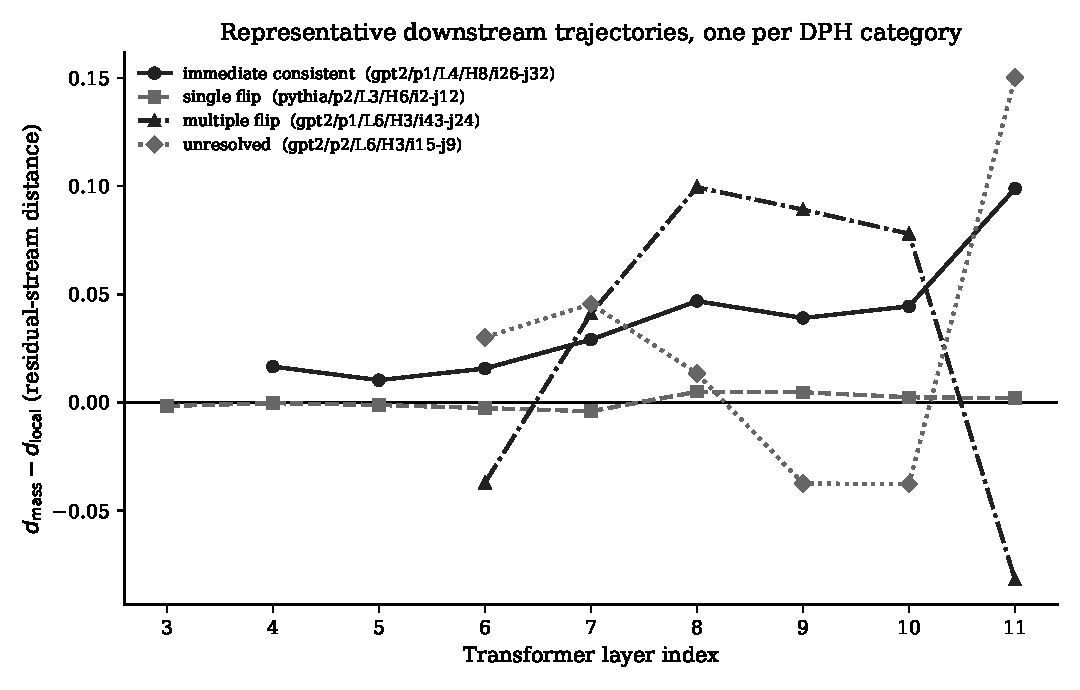
\includegraphics[width=0.85\textwidth]{figures/fig3_downstream_trajectories.pdf}
\caption{One representative case per DPH category, selected from the
250-case sample (\url{results/downstream_propagation_sample/cases.json})
by a fixed, documented rule: within each category, the case whose
$|\text{advantage}_{\text{final}}|$ is closest to that category's own
median (i.e.\ a case of typical, not maximal, effect size; ties broken by a
fixed architecture/prompt/layer/head/$i$/$j$ sort key). \emph{never\_consistent}
and \emph{unresolved} are pooled into one ``unresolved'' bucket, matching
Table~\ref{tab:dph}'s own convention. Selected cases: immediate\_consistent
= gpt2/p1/L4/H8/$i$26-$j$32; single\_flip = pythia/p2/L3/H6/$i$2-$j$12;
multiple\_flip = gpt2/p1/L6/H3/$i$43-$j$24; unresolved =
gpt2/p2/L6/H3/$i$15-$j$9 (full selection log, including each bucket's size
and median, in \url{manuscript/figures/FIGURE_PROVENANCE.md}). The
plotted quantity is each case's stored $d_{\text{mass}}-d_{\text{local}}$
residual-stream distance difference at every downstream layer, exactly as
defined in Section~\ref{sec:downstream}; no aggregation across cases. These
four trajectories are illustrative single examples ($n=1$ per category),
not distributional evidence; the distributional claims (flip rates and
their uncertainty) are Table~\ref{tab:dph}, not this figure.}
\label{fig:trajectories}
\end{figure}

Figure~\ref{fig:trajectories} shows one representative trajectory per
category, illustrating that the local ordering at the eviction layer can be
preserved, reversed once, reversed multiple times, or remain unresolved
through to the final layer.

\subsection{Local-vs-mass asymmetry}

\begin{table}[h]
\centering
\begin{tabular}{lcc}
\toprule
 & Local-final-winner ($n=126$) & Mass-final-winner ($n=124$) \\
\midrule
Flip rate & $0.206$ \; $[0.137,0.279]$ & $0.444$ \; $[0.347,0.543]$ \\
Immediate-consistent rate & $0.619$ \; $[0.519,0.711]$ & $0.242$ \; $[0.170,0.320]$ \\
\bottomrule
\end{tabular}
\caption{Subgroup cluster-bootstrap estimates by final downstream winner
(89 clusters for local-final-winner, 93 for mass-final-winner).}
\label{tab:localmass}
\end{table}

Cases where the exact local metric's preferred choice is also the final
downstream winner are, unsurprisingly, disproportionately
\emph{immediate\_consistent}; cases where attention-mass ultimately wins are
disproportionately associated with a flip. We report this as an
\textbf{empirical asymmetry requiring explanation}, not as a mechanism; no
experiment in this paper establishes why mass-final-winner cases flip more
often, and Section~\ref{sec:falsification}'s SDPH result specifically rules
out one tempting explanation (state-dependence) as the mechanism.

\section{Falsification of Candidate Explanations}
\label{sec:falsification}

Given Section~\ref{sec:downstream}'s result, we ask what \emph{does}
explain, or at least correlate with, whether a given case's immediate local
winner survives to become the downstream winner. Four candidate
explanations were tested, each motivated by the failure of the previous one;
this is a directed, sequential falsification program, not four independent
preregistered confirmatory trials, and we do not apply a multiple-comparisons
correction across them (Section~\ref{sec:discussion}).

\subsection{DVG: static directional value-vector geometry}

Eight cosine-similarity and norm-ratio features of the candidate value
vectors (e.g.\ $\cos(v_i,v_j)$, $\cos(v_i,o)$, $\cos(o-v_i,o-v_j)$) were
tested as predictors of the eventual winner, using pre-declared practical-weakness
thresholds ($|\text{AUC}-0.5|<0.05$ and $|r|<0.10$) rather than raw
significance. On Pythia ($n=1{,}962$ measurable pairs), the best grouped
cross-validated model reaches AUC $0.5496$ (vs.\ $0.5223$ for $|\Gamma|$
alone, $0.500$ for majority class); several features are statistically
detectable but fall below the pre-declared weakness threshold. On GPT-2
($n=22{,}477$, $\sim\!10\times$ the statistical power), the effect does not
strengthen: four of eight features remain near-zero despite the added power,
and zero of eight reach the within-stratum effect-size threshold. \textbf{Verdict:
static directional geometry fails to provide a replicated, useful predictor}
of the winner; the larger sample provides positive evidence against the
hypothesis, not merely an absence of significance.

\subsection{DPH: downstream propagation}

Reported in Section~\ref{sec:downstream}. \textbf{Verdict: propagation
through depth demonstrably produces substantial winner reversal (roughly
one third, cluster-aware), but does not follow a universal, cleanly
characterized rule} (e.g.\ emergence depth varies widely across cases; see
stored per-case trajectories).

\subsection{FLH: functional/logit-space representation}

We repeated the same trace, projecting hidden states to vocabulary space at
each layer (logit lens) and measuring KL divergence in output-distribution
space rather than residual-stream Euclidean distance, on the identical 250
cases (index-verified 1:1 reuse of the DPH sample, not an independent draw).
Cluster-aware paired differences (same resampled cells applied to both
analyses within each bootstrap replicate):
\[
\Delta_{\text{flip}} = \text{FLH} - \text{DPH} = -0.156,\quad
95\%\ \text{CI} = [-0.231,-0.082],
\]
\[
\Delta_{\text{unresolved}} = \text{FLH} - \text{DPH} = +0.392,\quad
95\%\ \text{CI} = [0.294, 0.485].
\]
Both intervals exclude zero. \textbf{We interpret this as functional space
trading fewer observed flips for substantially greater indeterminacy, not as
functional space resolving the ambiguity.} Consistent with this reading,
among the $56$ cases where residual space never stabilizes on the final
winner, functional space resolves only $35.7\%$ (95\% CI $[22.8\%,50.0\%]$)
of them --- still a minority. \textbf{Verdict: logit-space representation
does not resolve the residual-space ambiguity.}

\subsection{SDPH: state-dependent propagation}

Finally, we tested whether the \emph{same} downstream block responds
differently to an \emph{identical} perturbation depending on which policy's
trajectory produced its input state --- a targeted, causal swap-intervention
audit ($n=24$ hand-stratified cases, finite-difference scale sweep,
validation error $0.0$ against natural-forward reproduction). This effect is
real: it is present, close to linear in perturbation scale (relative
nonlinearity $\sim\!4$--$9\times10^{-4}$ across scales tested), and was
established causally, by intervention, not merely correlationally.

\textbf{This finding must not be read as an explanation for the DPH/FLH
reversals}, and we state the disconfirming evidence explicitly:
state-dependence does \emph{not} track flip status in the direction a
mechanistic story would predict. The pooled median state-dependence ratio
(flip cases vs.\ stable cases) is $0.2856$ --- \emph{flip cases show less}
measured state-dependence than stable cases, the opposite of what a
``state-dependence causes flips'' account would require. Architecture-split,
the pattern is inconsistent rather than confirmatory: Pythia shows
flip $\approx$ stable ($0.0712$ vs.\ $0.0702$ median $S$), while GPT-2 shows
flip $\ll$ stable ($0.0033$ vs.\ $0.0248$). \textbf{Verdict: state-dependence
is a confirmed, causally demonstrated phenomenon, but a falsified candidate
explanation for winner reversal} --- it exists, but not in the place or
pattern that would explain Sections~\ref{sec:downstream}'s result.

\subsection{Summary}

\begin{figure}[t]
\centering
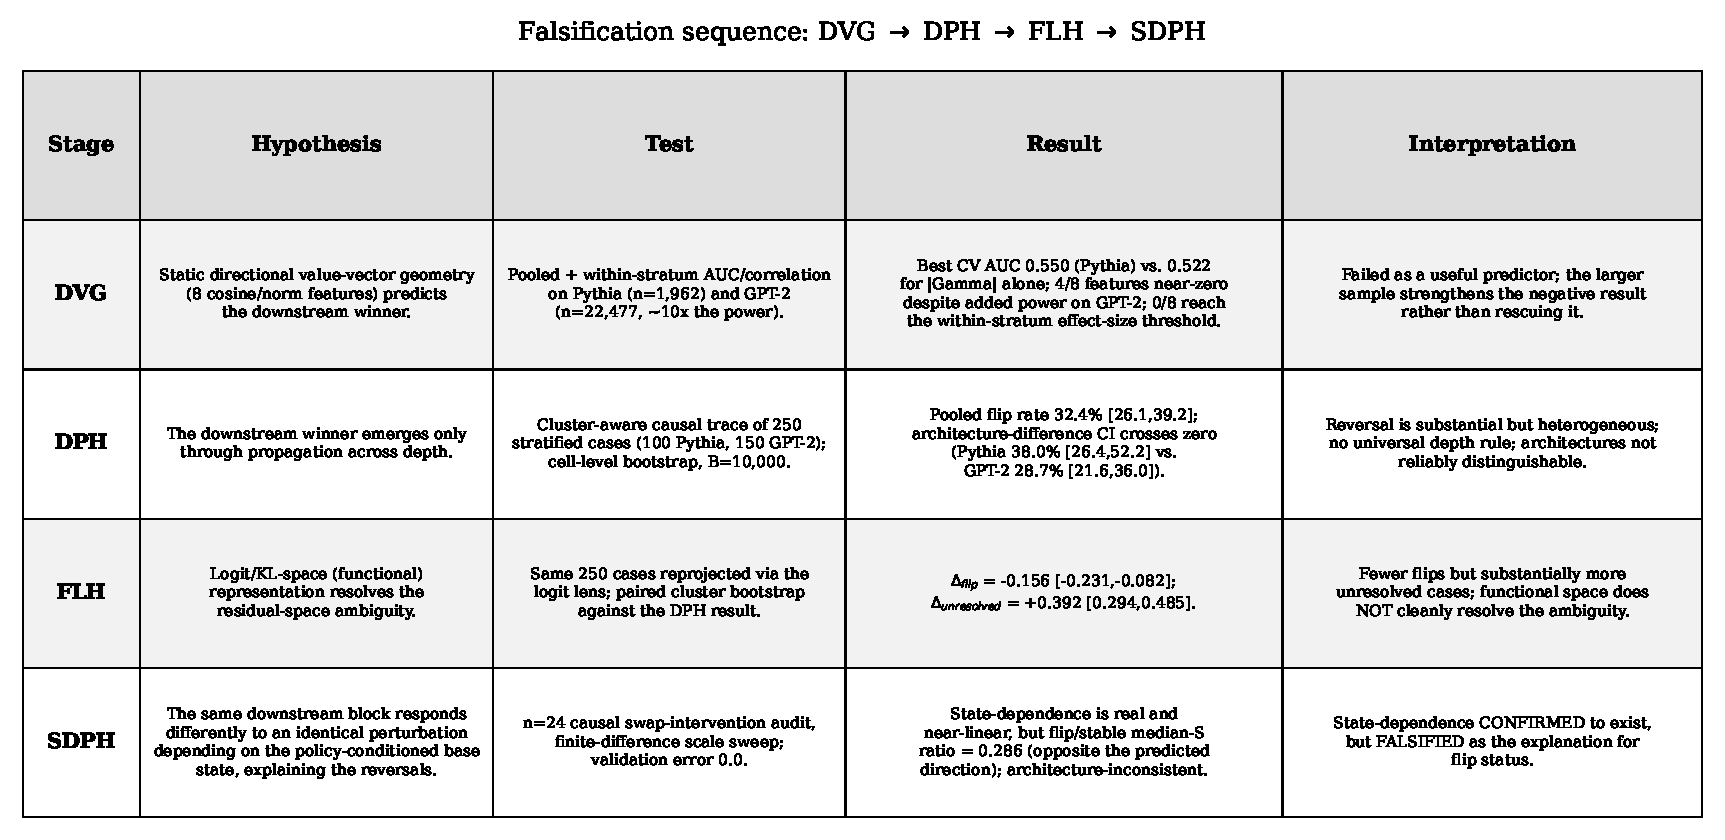
\includegraphics[width=\textwidth]{figures/fig4_falsification_summary.pdf}
\caption{The falsification sequence, hypothesis/test/result/interpretation
for each stage. Numbers reproduce exactly the conclusions stated in
Sections~\ref{sec:falsification}.1--\ref{sec:falsification}.4 above; no new
value is introduced here. The SDPH row deliberately states both that
state-dependence is confirmed to exist and that it is falsified as an
explanation for the DPH/FLH reversals, per the mandatory distinction
maintained throughout this section. Sources:
\url{results/directional_value_geometry/} and
\url{results/directional_value_geometry_gpt2/},
\url{results/cluster_aware_reanalysis/},
\url{results/state_dependent_propagation_audit/}; full derivation in
\url{manuscript/figures/FIGURE_PROVENANCE.md}.}
\label{fig:falsification}
\end{figure}

Figure~\ref{fig:falsification} summarizes the sequence.

\section{Discussion}
\label{sec:discussion}

\paragraph{On the simplicity of Theorem~\ref{thm:gamma}'s proof.} The proof
of the $\Gamma$ boundary is two lines of algebra: dividing one positive
quantity by another and taking a monotone log transform. We do not dispute
that this is mathematically simple, and we do not claim depth of derivation
as the contribution. What Theorem~\ref{thm:gamma} does is convert a
question that could otherwise only be answered empirically, case by case
("does the local-perturbation ranking agree with the attention-mass ranking
here?"), into a closed-form condition that can be checked exactly and at
scale -- which is what makes the $482{,}787$-pair verification of
Section~\ref{sec:design} and the four-stage falsification program of
Section~\ref{sec:falsification} possible in the first place. The paper's
substance, in other words, is claimed to lie in the empirical and causal
program the boundary condition enables, not in the algebra itself.

The overall picture is that exact local information about a KV-cache
eviction decision is genuinely exact --- Theorem~\ref{thm:delta} is an
identity, not an approximation, and Theorem~\ref{thm:gamma} gives a provably
correct boundary for when two natural rankings of that local information
disagree --- and that this exactness does not transfer to the downstream
question practitioners usually care about. None of the four candidate
mechanisms we tested reduces the downstream behavior to something simply
characterized in terms of quantities available at eviction time. The one
positive causal finding among them (state-dependence, SDPH) is real but
points \emph{away from} a simple explanation, since its pattern does not
track which cases flip.

On the sequential-hypothesis question: DVG, DPH, FLH, and SDPH were run in
sequence, each motivated by the previous stage's outcome, several of them
using pre-declared effect-size thresholds rather than a single significance
gate, and FLH/SDPH partially reuse the DPH sample (explicitly disclosed
above, not concealed). We treat this as a directed falsification narrative,
not four independent preregistered confirmatory trials, and accordingly do
not apply a Bonferroni-style correction across them; we do report
cluster-aware, rather than naive i.i.d., uncertainty for every quantity
where case non-independence is plausible.

\section{Limitations}
\label{sec:limitations}

\begin{itemize}[nosep]
\item Two architectures only (Pythia-160M, GPT-2 124M), both small by
current standards; no modern instruction-tuned or much larger model is
tested.
\item The Pythia grid (55{,}971 pairs, 5 layers $\times$ 4 heads) and the
GPT-2 grid (426{,}816 pairs, full 12 $\times$ 12) differ in density and
coverage; the reported prevalence difference is not a controlled comparison.
\item The 250-case downstream sample is stratified by design; reported
rates describe the stratified sample's cluster-aware behavior, not raw
unweighted prevalence across all measurable inversions.
\item Some subgroup/cluster analyses (notably Pythia-only, 34 clusters, 9
singleton) have wide intervals and should not be over-interpreted;
architecture differences in particular are not established (CI crosses
zero throughout).
\item ``Measurable'' KL differences are defined relative to a pre-declared
numerical noise floor; this establishes the effect is not numerical noise,
not that it is practically significant for any downstream task.
\item We do not evaluate any policy against deployed eviction systems
(H$_2$O, SnapKV, StreamingLLM, etc.) on task quality; this paper makes no
claim about which policy one should deploy.
\item Logit-lens-based measurements carry float32 reconstruction noise
(bounded at $2.2\times10^{-5}$ against true final-layer KL in our
validation), handled by a diagnostically justified tolerance
($10^{-4}$), not a tolerance chosen to fit the result.
\end{itemize}

\section{Conclusion}
\label{sec:conclusion}

We derived an exact, closed-form pairwise boundary for when attention-mass
and exact local-output-perturbation rankings of KV-cache eviction candidates
disagree, built on a singleton identity that we explicitly do not claim as
novel (it is algebraically identical to prior KeepKV work
\cite{keepkv2025}). Across two architectures, such disagreements are common,
almost always change the eviction decision, and almost always produce a
measurable downstream effect --- yet the locally preferred choice is
overturned by later computation in roughly a third of cluster-aware sampled
cases, and a four-stage falsification program finds no simple predictor of
when. Exact local correctness, in other words, is not the same thing as
downstream predictive power, and this paper's evidence is a specific,
quantified account of that gap for one narrow but concrete setting, not a
general claim about transformers.

\appendix

\section{Figure Status}
\label{app:figures}

This appendix records where each main-paper figure lives and how it was
produced.

\begin{small}
\begin{enumerate}[nosep]
\item \textbf{Exact local eviction geometry and the $\Gamma=0$ boundary} ---
Figure~\ref{fig:local-gamma}, Section~\ref{sec:gamma}. Schematic (synthetic
numeric example run through the real formulas of
Theorems~\ref{thm:delta}/\ref{thm:gamma}); no stored result file is used.
Region labels compare only which of two candidates has the larger exact
local perturbation ($d_i>d_j$ vs.\ $d_i<d_j$), not which eviction policy
wins downstream.
\item \textbf{Inversion $\to$ set-change $\to$ measurable-KL chain} ---
Figure~\ref{fig:inversion-chain}, Section~\ref{sec:consequences}.
Data-derived from \url{results/full_grid_mechanistic_analysis/} (Pythia) and
\url{results/cross_architecture_full_grid/} (GPT-2), recomputed directly by
the generating script rather than transcribed. Reports Section~\ref{sec:consequences}
statements (1)--(3) only; statement (4) is Figure~\ref{fig:trajectories}.
\item \textbf{Representative downstream trajectories} ---
Figure~\ref{fig:trajectories}, Section~\ref{sec:downstream}. Data-derived
from \url{results/downstream_propagation_sample/cases.json}; one case per
category selected by a fixed median-magnitude rule, documented in full in
\url{manuscript/figures/FIGURE_PROVENANCE.md}.
\item \textbf{Falsification summary (DVG$\to$DPH$\to$FLH$\to$SDPH)} ---
Figure~\ref{fig:falsification}, Section~\ref{sec:falsification}. Renders,
with no new numbers, the conclusions already stated in
Section~\ref{sec:falsification}'s four subsections; supersedes an earlier
3-column LaTeX table with a 4-column (hypothesis/test/result/interpretation)
layout.
\end{enumerate}
\end{small}

Generation script: \url{manuscript/figures/generate_figures.py} (requires
only already-stored result files and \texttt{matplotlib}; performs no model
forward pass). Full per-figure provenance --- exact source file, result
keys, filters, case IDs, and any aggregation --- is in
\url{manuscript/figures/FIGURE_PROVENANCE.md}.

\section{Supplementary Material Not Reproduced in the Main Text}
\label{app:supplement}

The main text is deliberately restricted to the theorem-to-downstream
narrative. The following material exists in the project's stored results
but is intentionally not reproduced in the main text; a future appendix
pass should draw directly from these files rather than re-deriving numbers:

\begin{small}
\begin{itemize}[nosep]
\item \textbf{Full adapter validation detail} beyond the summary figures
quoted in Section~\ref{sec:design}: \url{results/cross_architecture_generalization/report.txt},
\url{tests/test_gpt2_adapter.py}.
\item \textbf{Full architecture grids} (per-cell counts, strongest pairs,
percentile tables): Pythia in
\url{results/full_grid_mechanistic_analysis/summary.json}; GPT-2 in
\url{results/cross_architecture_full_grid/summary.json} (report at
\url{results/cross_architecture_full_grid/report.txt}).
\item \textbf{Per-stratum heterogeneity} (Gini coefficient of inversions
across cells, strongly mass-/local-favoring strata, concentration-vs-prevalence
correlations): \url{results/cross_architecture_full_grid/report.txt}.
\item \textbf{The 36-cell GPT-2 pilot grid}, used only for adapter
validation in the main text (Section~\ref{sec:design}): full pilot report at
\url{results/cross_architecture_generalization/report.txt}. Its own
prevalence estimate (6.62\%, a third, smaller grid with different
layer/head coverage than either headline grid) is recorded there but is not
a headline result of this paper.
\item \textbf{Extended DVG feature detail} (all 8 directional features,
pooled/within-stratum statistics, tail-case audits, minimal multivariate
models): \url{results/directional_value_geometry/report.txt},
\url{results/directional_value_geometry_gpt2/report.txt}.
\item \textbf{FLH residual-vs-functional cross-tabulation} (the full
2$\times$2 breakdown underlying the ``resolves 35.7\% of never-consistent
cases'' statistic) and per-layer KL/JS/L2/cosine detail:
\url{results/functional_propagation_audit/report.txt},
\url{results/functional_propagation_audit/cases.json}.
\item \textbf{SDPH linearity controls} (state-dependence $S$ at multiple
perturbation scales, attention-vs-MLP component audit, per-architecture
breakdowns): \url{results/state_dependent_propagation_audit/report.txt}.
\item \textbf{Cluster-bootstrap sensitivity analyses} (alternate cluster
definitions: layer$\times$head collapsing architecture and prompt;
architecture$\times$prompt collapsing layer and head): the
\texttt{sensitivity\allowbreak\_alternate\allowbreak\_cluster\allowbreak\_definitions}
key of \url{results/cluster_aware_reanalysis/summary.json}.
\end{itemize}
\end{small}

\section*{Acknowledgments}

This work was developed through an integrated human--AI research workflow.
The author directed the research program, formulated the central questions
and hypotheses, evaluated the mathematical and empirical results, and
retained responsibility for all scientific claims and conclusions. Claude
(Anthropic) was used extensively for repository-based implementation,
computational experimentation, formal auditing, statistical analysis,
literature-assisted review, figure generation, and manuscript development.
ChatGPT (OpenAI) was used for research planning, mathematical and
conceptual analysis, interpretation of experimental results, critical
evaluation of claims, manuscript strategy, and iterative synthesis across
the research program. Both AI systems contributed substantially to the
research process as interactive computational and reasoning tools. The
author reviewed and approved the resulting mathematics, experiments, code,
interpretations, and manuscript and assumes responsibility for the final
work.

\begin{thebibliography}{9}

\bibitem{keepkv2025}
Yuxuan Tian, Zihan Wang, Yebo Peng, Aomufei Yuan, Zhiming Wang, Bairen Yi,
Xin Liu, Yong Cui, Tong Yang.
\newblock KeepKV: Achieving Periodic Lossless KV Cache Compression for
Efficient LLM Inference.
\newblock \emph{arXiv preprint arXiv:2504.09936}, 2025.
\newblock (No conference/venue acceptance is stated on the arXiv page as of
this citation; cited as an arXiv preprint only.)

\bibitem{h2o2023}
Zhenyu Zhang, Ying Sheng, Tianyi Zhou, Tianlong Chen, Lianmin Zheng, Ruisi
Cai, Zhao Song, Yuandong Tian, Christopher R\'e, Clark Barrett, Zhangyang
Wang, Beidi Chen.
\newblock H$_2$O: Heavy-Hitter Oracle for Efficient Generative Inference of
Large Language Models.
\newblock \emph{arXiv preprint arXiv:2306.14048}, 2023. NeurIPS 2023.

\bibitem{scissorhands2023}
Zichang Liu, Aditya Desai, Fangshuo Liao, Weitao Wang, Victor Xie, Zhaozhuo
Xu, Anastasios Kyrillidis, Anshumali Shrivastava.
\newblock Scissorhands: Exploiting the Persistence of Importance Hypothesis
for LLM KV Cache Compression at Test Time.
\newblock \emph{arXiv preprint arXiv:2305.17118}, 2023. NeurIPS 2023.

\bibitem{streamingllm2024}
Guangxuan Xiao, Yuandong Tian, Beidi Chen, Song Han, Mike Lewis.
\newblock Efficient Streaming Language Models with Attention Sinks.
\newblock \emph{arXiv preprint arXiv:2309.17453}, 2023. ICLR 2024.

\bibitem{criticalkv2025}
Yuan Feng, Junlin Lv, Haoyu Guo, Yukun Cao, S Kevin Zhou, Xike Xie.
\newblock CriticalKV: Optimizing KV Cache Eviction from an Output
Perturbation Perspective.
\newblock \emph{arXiv preprint arXiv:2502.03805}, 2025.

\bibitem{fixedcontract2026}
Ruijie Zhang, Haozhe Liang, Da Chang, Li Hu, Fanqi Kong, Huaxiao Yin, Yu Li.
\newblock When Does Value-Aware KV Eviction Help? A Fixed-Contract
Diagnostic for Non-Monotone Cache Compression.
\newblock \emph{arXiv preprint arXiv:2605.08234}, 2026.

\bibitem{rome2022}
Kevin Meng, David Bau, Alex Andonian, Yonatan Belinkov.
\newblock Locating and Editing Factual Associations in GPT.
\newblock \emph{Advances in Neural Information Processing Systems (NeurIPS)},
2022. arXiv:2202.05262.

\bibitem{tunedlens2023}
Nora Belrose, Igor Ostrovsky, Lev McKinney, Zach Furman, Logan Smith, Danny
Halawi, Stella Biderman, Jacob Steinhardt.
\newblock Eliciting Latent Predictions from Transformers with the Tuned
Lens.
\newblock \emph{arXiv preprint arXiv:2303.08112}, 2023.

\end{thebibliography}

\end{document}
